\subsection{Currency Exchange Rates}

\begin{definition} \hlt{Exchange Rate}\\
Price of one currency in terms of another.\\
Typically quoted as 'Price/Base' notation, i.e., $1.650$ USD/EUR means $1$ EUR cost $1.650$ USD.
\begin{enumerate}[label=\roman*.]
\setlength{\itemsep}{0pt}
\item Spot exchange rate: for immediate delivery, with $T+2$ settlement (except CAD/USD, with $T+1$)
\item Forward exchange rate: to be done in future.
\end{enumerate}
\end{definition}

\begin{remark} \hlt{Dealer Quotes}\\
Quoted as 'Bid-Ask', where bid price is price at which dealer will buy, ask is price at which dealer sells.
\end{remark}

\begin{remark} \hlt{Foreign Exchange Spread}\\
Difference between offer and bid price is the spread, quoted as 'pips', which is $1/10,000$ of a dollar.\\
Ask Price $>$ Bid Price. Bid-offer spread from dealer is wider than the spread dealer receives from interbank.
\end{remark}

\begin{remark} \hlt{Dealer Spread Factors}
\begin{enumerate}[label=\roman*.]
\setlength{\itemsep}{0pt}
\item Spread in interbank market: spreads vary directly with spreads quoted in interbank market.
\item Size of transaction: large, liquidity-demanding transactions get quoted larger spread.
\item Relationship between dealer and client: dealer give favourable rates to preferred clients based on other ongoing business relationships.
\end{enumerate}
\end{remark}

\begin{remark} \hlt{Interbank Spread Factors}
\begin{enumerate}[label=\roman*.]
\setlength{\itemsep}{0pt}
\item Currencies traded: high-volume currency pairs command lower spreads than lower-volume pairs
\item Time of day: most liquid when major trading centres are open (Asian session not as liquid as London, NY sessions). Spreads are narrower when both NY, London sessions are open.
\item Market volatility: higher volatility due to geopolitical events, market crashes, major data releases will lead to wider spreads. Spreads change over time in response to volatility changes.
\end{enumerate}
\end{remark}

\begin{remark} \hlt{Forward Exchange Rate Spreads}\\
Spreads in forward exchange rate quotes increase with maturity, as:
\begin{enumerate}[label=\roman*.]
\setlength{\itemsep}{0pt}
\item longer maturity contracts tend to be less liquid,
\item counterparty credit risk in forward contracts increase with maturity,
\item interest rate risk in forward contracts increase with maturity
\end{enumerate} 
\end{remark}

\begin{remark} \hlt{Tips with Foreign Transaction Quotes}
\begin{enumerate}[label=\roman*.]
\setlength{\itemsep}{0pt}
\item For transactions in base currency, buy base currency at ask, sell base currency at bid.
\item For transactions in price currency, buy price currency at bid, sell price currency at ask.
\item Alternatively, follow the up-the-bid-and-multiply, down-the-ask-and-divide rule.\\
i.e., given USD/AUD, to convert USD into AUD, use ask (going down the quote).\\
To convert AUD to USD, use bid (going up the quote).
\end{enumerate}
\end{remark}

\begin{definition} \hlt{Cross Rate}\\
Exchange rate between two currencies implied by exchange rates with a common third currency.\\
To use cross rates when there is no active FC market in currency pair considered.
\end{definition}

\begin{remark} \hlt{Cross Rates with Bid-Ask Spreads}\\
Bid-ask spreads complicate the computation of cross rates. Suppose we have currencies $A,B,C$.
\begin{align}
\left(\frac{A}{C} \right)_{\text{Bid}} &= \left(\frac{A}{B} \right)_{\text{Bid}} \times \left(\frac{B}{C} \right)_{\text{Bid}}, \ \ \ \ \ \ \ \ \ \ \left(\frac{A}{C} \right)_{\text{Offer}}  = \left(\frac{A}{B} \right)_{\text{Offer}} \times \left(\frac{B}{C} \right)_{\text{Offer}} \nonumber
\end{align}
If given instead $A/B$ and $C/B$ rates, make adjustments to obtain $B/C$ bid and offer rates from $C/B$ bid and offer rates, as $A/B \times C/B \neq A/C$. Process is
\begin{align}
\left(\frac{B}{C} \right)_{\text{Bid}} = \frac{1}{\left(\frac{C}{B} \right)_{\text{Offer}}}, \ \ \ \ \ \ \ \left(\frac{B}{C} \right)_{\text{Offer}} = \frac{1}{\left(\frac{C}{B} \right)_{\text{Bid}}} \nonumber
\end{align}
\end{remark}

\begin{method} \hlt{Triangular Arbitrage}\\
Begin with tree pairs of currencies, each with bid-ask quotes, construct a triangle where each node in triangle represents one currency. To check for arbitrage, go around the triangle clockwise (and counterclockwise) until starting point. Follow the up-the-bid-and-multiply, down-the-ask-and-divide rule.\\
Only one direction is profitable; cannot earn arbitrage profit in both directions.
\end{method}

\begin{figure}[H]
\centering
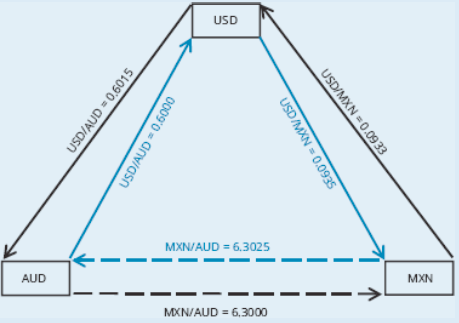
\includegraphics[scale=0.5]{/econ/trianglearb}
\caption{Example of triangle arbitrage, only blue is profitable}
\end{figure}

\begin{definition} \hlt{Forward Rates}\\
Currency is quoted at forward premium (discount) relative to second currency if forward price is greater (less) than spot price. The premium or discount is for the base currency.
\begin{equation}
\text{Forward Premium} = F_{f/d} - S_{f/d} \nonumber
\end{equation}
In FX markets, forward quotes are presented as premium or discount over spot rates.\\
Note, spot rate $S_{f/d}$ is mid-market of bid-offer spread.
\end{definition}

\begin{remark} \hlt{Mark-to-Market Value}\\
Value of forward contract prior to expiration is also known as mark-to-market value.\\
Take difference between forward price locked-in and currency forward price, multiply that by size of contract, then discount for time remaining until contract settlement date.
\begin{equation}
V_t = \frac{(F_t - F_0)(\text{Contract Size})}{1 + i_f(\frac{n}{360})} \nonumber
\end{equation}
where $i_f$ is interest rate (MRR) of price currency, $n$ is days remaining to maturity of contract ($T-t$).\\
Note the forward price is to sell base currency, and MRR is market reference rate.
\end{remark}

\subsubsection{International Parity Conditions}

\begin{remark} \hlt{Relationship of Forward Rate to Spot Rates}\\
Given one unit of domestic currency, two investment choices may be made:
\begin{enumerate}[label=\roman*.]
\setlength{\itemsep}{0pt}
\item Invest in cash for $1$ year at domestic risk-free rate to earn $1 + i_d$.
\item Convert domestic currency to foreign currency at spot rate $S_{f/d}$, invest for one year at foreign risk-free rate $i_f$, then at end of period, will have $S_{f/d}(1+i_f)$ units of foreign currency.\\
Convert back at forward rate of $F_{f/d}$, then we would have $S_{f/d}(1+i_f)(1/F_{f/d})$ units of domestic currency.
\end{enumerate}
As both are risk free, should offer same return, hence we have the relationship
\begin{equation}
(1+i_d) = S_{f/d} (1+i_f) \left( \frac{1}{F_{f/d}} \right) \nonumber
\end{equation}
\end{remark}

\begin{definition} \hlt{Covered Interest Rate Parity}\\
'Covered' means bound by arbitrage; arbitrage force forward contract exchange rate to a level consistent with difference between two country's nominal interest rates.\\
Parity holds when any forward premium or discount exactly offsets differences in interest rates, hence investor would earn the same return in either currency.\\
If foreign interest rates are higher than local interest rates, the forward discount on foreign currency relative to local currency will just offset the higher foreign interest rate.
\begin{align}
F_{f/d} = S_{f/d} \left( \frac{1 + i_f (\frac{n}{360})}{1 + i_d (\frac{n}{360})} \right), \ \ \ \ \ \  \text{Forward Premium} = F_{f/d} -  S_{f/d} = S_{f/d} \left( \frac{(\frac{n}{360})}{1 + i_d (\frac{n}{360})} \right) (i_f - i_d) \nonumber
\end{align}
\end{definition}

\begin{definition} \hlt{Uncovered Interest Rate Parity}\\
'Uncovered' means not bound by arbitrage. If forward contracts are not available, or if capital flows are restricted so as to prevent arbitrage, then the relationship need not hold.\\
Given $f/d$, the base currency $d$ is expected to appreciate by approximately $i_f - i_d$.
\begin{equation}
\% \Delta S^e_{f/d} = i_f - i_d \nonumber
\end{equation}
where $\% \Delta S^e_{f/d}$ is change in spot rate expected.\\
There is no reason that uncovered interest rate parity must hold in short run.\\
There is evidence that it does generally hold in the long-run, hence longer-term expected future spot rate based on uncovered parity are often used as future exchange rate forecasts.
\end{definition}

\begin{remark} \hlt{Covered vs Uncovered Interest Rate Parity}
\begin{enumerate}[label=\roman*.]
\setlength{\itemsep}{0pt}
\item Covered parity derives the no-arbitrage forward rate, while uncovered parity derives the expected future spot rate (which is not market traded).
\item Under uncovered parity, if foreign interest rate is higher, foreign currency is expected to depreciate by approximately same amount, hence investor is indifference between investing in foreign or domestic currency. An investor that chooses to invest to foreign currency without additional return is not demanding a risk premium for foreign currency risk. Hence uncovered parity assumes investor is \hlt{risk-neutral}.
\end{enumerate}
\end{remark}

\begin{definition} \hlt{Forward Rate Parity}\\
If covered interest rate parity holds, and uncovered interest rate parity also holds; where the no-arbitrage forward rate equals the expected future spot rate.
\begin{equation}
\frac{F_{f/d} - S_{f/d}}{S_{f/d}} = \% \Delta S^e_{f/d} = i_f - i_d \nonumber
\end{equation}
Hence $F_{f/d} = S_{f/d, t}^e$. The forward rate is an unbiased predictor of future spot rate.
\end{definition}

\begin{definition} \hlt{(Domestic) Fisher Relation}\\
Nominal rate of return is approximately the sum of real rate and expected rate of inflation.
\begin{equation}
i = r + \pi^e \nonumber
\end{equation}
\end{definition}

\begin{definition} \hlt{Real Interest Rate Parity}\\
Real interest rates will converge to same level across different markets.
\begin{equation}
r_f - r_d = 0 \nonumber
\end{equation}
\end{definition}

\begin{definition} \hlt{International Fisher Effect}\\
Taking domestic fisher relation and real interest rate parity together; difference between two countries' nominal interest rates should be equal to difference between their expected inflation rates.
\begin{equation}
i_f - i_d = \pi_f^e - \pi_d^e \nonumber
\end{equation}
Argument for equality of real interest rates across countries is based on idea that free capital flows, funds will move to a country with higher real rate until real rates are equalised.
\end{definition}

\begin{definition} \hlt{Law of One Price}\\
Identical goods should trade at the same price across countries when valued in terms of a common currency.
\end{definition}

\begin{definition} \hlt{Absolute Purchasing Power Parity (Absolute PPP)}\\
Compares average price of representative basket of consumption goods between countries using an index.\\
Requires only that the law of once price be correct on average. Assumes goods arbitrage will equate prices of all goods and services across countries.
\begin{equation}
S_{f/d} = \frac{P_f}{P_d} \nonumber
\end{equation}
In practice, even of law of one price holds, absolute PPP might not hold as weights (consumption patterns) of various goods in two economies may not be the same.
\end{definition}

\begin{definition} \hlt{Relative Purchasing Power Parity (Relative PPP)}\\
Changes in exchange rates should exactly offset the price effects of any inflation differential between two countries. Assumes transaction costs and other trade impediments are constant over time.
\begin{equation}
\% \Delta S_{f/d} = \pi_f - \pi_d \nonumber
\end{equation}
Based on idea that even if absolute PPP does not hold, there may still be a relationship between changes in exchange rate and differences between inflation rates of two countries.\\
As there is no true arbitrage available to force relative PPP to hold, violations of relative PPP in short run are common. However, evidence suggests that relative PPP holds approximately in the long-run, and remains a useful method for estimating relationship between exchange rates and inflation rates.
\end{definition}

\begin{definition} \hlt{Ex-Ante Purchasing Power Parity (Ex-Ante PPP)}\\
Same as relative PPP, except it uses expected inflation instead of actual inflation.\\
Countries with persistently high inflation rates should expect to see their currencies depreciate.
\begin{equation}
\% \Delta S_{f/d}^e = \pi_f^e - \pi_d^e \nonumber
\end{equation}
\end{definition}

\begin{figure}[H]
\centering
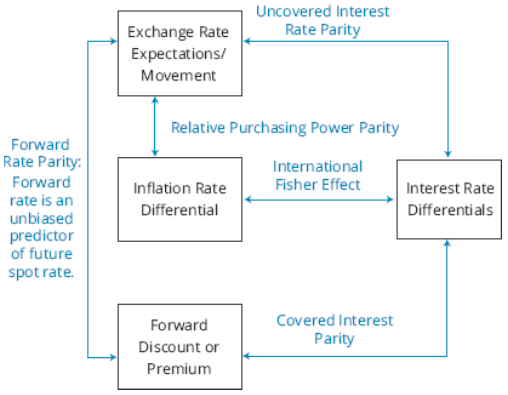
\includegraphics[scale=0.523]{/econ/intparity}
\caption{Relationship between international parity conditions}
\end{figure}

\begin{remark} \hlt{Summary of International Parity Conditions}
\begin{enumerate}[label=\roman*.]
\setlength{\itemsep}{0pt}
\item Covered interest rate parity: arbitrage ensures nominal i/r spread = \% forward premium
\item Uncovered interest rate parity: expected $\% \Delta$ spot rate = nominal i/r spread
\item If covered and covered parity holds, then forward rate is unbiased predictor of future spot rate
\item Ex ante PPP: expected $\Delta$ spot rate = expected diff in domestic and foreign i/r
\item Fisher effect: nominal i/r = real i/r $+$ expected inflation rate; real i/r parity holds
\item International fisher effect: nominal yield spread $=$ domestic and foreign i/r expected inflation differential
\item If ex ante PPP, international fisher effect hold, then expected inflation diff = expected change in exchange rate and nominal i/r differential.\\
Relationship implies expected $\Delta$ exchange rate $=$ nominal i/r diff (uncovered i/r parity)
\end{enumerate}
\end{remark}

\begin{remark} \hlt{Observations of Relationship of Parity Conditions}
\begin{enumerate}[label=\roman*.]
\setlength{\itemsep}{0pt}
\item Covered interest rate parity holds by arbitrage. If forward rate parity holds, uncovered interest rate parity also holds (and vice versa)
\item Interest rate differentials should mirror inflation differentials. This holds true if the international Fisher relation holds. If that is true, can also use inflation differentials to forecast future exchange rates, which is the premise of ex-ante PPP.
\item If ex-ante PPP and international Fisher relation both hold, uncovered interest rate parity will also hold.
\end{enumerate}
\end{remark}

\begin{remark} \hlt{All Parity Condition Holds}\\
If all key international parity conditions hold at all times, $\Delta$ spot rate equals:
\begin{enumerate}[label=\roman*.]
\setlength{\itemsep}{0pt}
\item forward premium or discount (in percentage terms)
\item nominal yield spread between countries
\item difference between expected national inflation rates
\end{enumerate}
Impossible for global investor to earn consistent profit on forex movements.
\end{remark}

\begin{definition} \hlt{FX Carry Trade}\\
Long high-yield currencies, short low-yield currencies. Bets that high-yield currencies have not depreciated and low-yield currencies have not appreciated to levels predicted by interest rate differentials.\\
Strategy can be executed as uncovered interest parity does not hold over short, medium term periods.\\
Strategy attempts to capture interest rate differential, and is a bet against uncovered interest rate parity.\\
Carry trades perform well in low-volatility periods. Higher yields attract larger capital flows, lead to economic boom and appreciation of higher-yield currency, hence earning currency appreciation and interest rate spread. 
\end{definition}

\begin{remark} \hlt{Risks of FX Carry Trade}\\
Risk is that the funding currency may appreciate significantly against investment currency, leading to loss.\\
Return distribution is not normal, with negative skewness and excess kurtosis (fat tails), hence there is a high probability of a large loss (crash risk), this stems from carry trade's leveraged nature.
\end{remark}

\subsubsection{Central Bank Influence}

\begin{definition} \hlt{Balance-of-Payments (BOP) Accounting}\\
Method used to keep track of transactions between country and trading partners.\\
Includes government transactions, consumer transactions, and business transactions.\\
Accounts reflect all payments and liabilities to and from foreigners.
\end{definition}

\begin{definition} \hlt{Current Account}\\
Measures exchange of goods and services, investment income, and unilateral transfers (gifts).
\end{definition}

\begin{definition} \hlt{Financial Account}\\
Measures the flow of funds for debt and equity investment into and out of the country.
\end{definition}

\begin{remark} \hlt{Relationship between Current Account and Capital Account}\\
With current account deficit, to generate a surplus in capital account (or currency will depreciate).\\
Capital flows tend to be the dominant factor influencing exchange rates in the short term, as capital flows tend to be larger and more rapidly changing than goods flows.
\end{remark}

\begin{remark} \hlt{Current Account Influences on Exchange Rates}
\begin{enumerate}[label=\roman*.]
\setlength{\itemsep}{0pt}
\item Flow Supply/Demand Channel: if country sold more goods and services than it purchased (current account surplus), demand for currency should rise, hence appreciate.\\
Assumes trade imbalances will be corrected as deficit country’s currency depreciates.\\
Amount by which exchange rate adjusts depends on
\begin{enumerate}[label=\arabic*.]
\setlength{\itemsep}{0pt}
\item Initial surplus: larger surplus requires larger appreciation of domestic currency
\item Influence of exchange rates on domestic import and export prices
\item Price elasticity of demand of traded goods 
\end{enumerate}
\item Portfolio Balance Channel: country with current account surpluses have capital account deficits, which are investments in countries with current account deficits. Due to flows of capital, investor countries portfolio composition is dominated by few investee currencies. When investor rebalance portfolios, it may have significant negative impact on value of investee country currencies.
\item Debt Sustainability Channel: country with current account deficit is running a current account surplus by borrowing from abroad. When level of debt is too high relative to GDP, investors may question sustainability of debt level, leading to rapid depreciation of borrower currency.
\end{enumerate}
\end{remark}

\begin{remark} \hlt{Capital Account Influences on Exchange Rates}\\
As capital flows into country, demand for currency increases, resulting in appreciation.\\
Higher relative real rates of return attract foreign capital. Capital flows into a country may be needed to overcome shortage of internal savings to fund investments. However, capital flows in excess of needed investment capital pose several problems:
\begin{enumerate}[label=\roman*.]
\setlength{\itemsep}{0pt}
\item Excessive real appreciation of the domestic currency,
\item Financial asset and/or real estate bubbles.
\item Increases in external debt by businesses or government. 
\item Excessive consumption in the domestic market fuelled by credit.
\end{enumerate}
Emerging market governments counteract excessive capital inflows by imposing capital controls or by direct intervention in the foreign exchange markets.
\end{remark}

\begin{definition} \hlt{Mundell-Fleming Model}\\
Model evaluates the short-term impact of monetary and fiscal policies on interest rates, exchange rates.\\
Assumes there is sufficient slack in economy to handle changes in aggregate demand, and inflation is not concern.\\
Changes in inflation rates play no role in exchange rate determination.
\end{definition}

\begin{remark} \hlt{Mundell-Fleming Model: Flexible Exchange Rate Regimes}\\
Rates are determined by supply and demand in FX markets. 
\begin{enumerate}[label=\roman*.]
\setlength{\itemsep}{0pt}
\item High Capital Mobility:
\begin{enumerate}[label=\arabic*.]
\setlength{\itemsep}{0pt}
\item Expansionary monetary policy reduce interest rate, and hence reduce inflow of capital investment in physical and financial assets, hence reduces demand for domestic currency, resulting in appreciation of domestic currency. Vice versa for restrictive monetary policy.
\item Expansionary fiscal policy increase government borrowing and hence increase interest rates, attracting foreign investment, improve financial account, increase demand for currency. Vice versa for restrictive.
\end{enumerate}
\item Low Capital Mobility: impact of trade imbalance on exchange rates is greater than impact of interest rates. Expansionary fiscal or monetary policy leads to increases in net imports, leading to depreciation.
\end{enumerate}
\end{remark}

\begin{flushleft}
Monetary and Fiscal Policy and Exchange Rates
\begin{tabularx}{\textwidth}{p{10em}|p{10em}|X|X}
\hline
\rowcolor{gray!30}
Monetary Policy & Fiscal Policy & High Capital Mobility & Low Capital Mobility\\
\hline
Expansionary & Expansionary & Uncertain & Depreciation\\
\hline
Expansionary & Restrictive & Depreciation & Uncertain\\
\hline
Restrictive & Expansionary & Appreciation & Uncertain\\
\hline
Restrictive & Restrictive & Uncertain & Appreciation\\
\hline
\end{tabularx}
\end{flushleft}

\begin{remark} \hlt{Mundell-Fleming Model: Fixed Exchange Rate Regime}\\
Expansionary monetary policy will lead to depreciation of domestic currency. Government to purchase own currency in FX market, reversing the expansionary stance.\\
Hence, governments cannot both management exchange rates and pursue independent monetary policy. If government wants to manage 
\end{remark}

\begin{definition} \hlt{Monetary Approach to Exchange Rate Determination}\\
Assume that output is fixed, so monetary policy primarily affects inflation, which affects exchange rates.
\begin{enumerate}[label=\roman*.]
\setlength{\itemsep}{0pt}
\item Pure Monetary Model: PPP holds at any point in time, output is held constant. Expansionary monetary policy results in $x \% \uparrow$ money supply, hence  $x \% \uparrow$ in price levels, and an  $x \%$ depreciation of currency.\\
Approach does not take into account expectations on future monetary expansion or contraction.
\item Dornbusch Overshooting Model: assumes prices are sticky in short term, hence do not immediately reflect changes in monetary policy (PPP does not hold in short term). Exchange rates will overshoot long-run PPP value in short term. Expansionary monetary policy increase prices, but in over time leads to a decrease in interest rates, and a larger-than-PPP-implied depreciation of domestic currency due to capital inflows. In long run, exchange rates gradually increase towards PPP implied values.
\end{enumerate}
\end{definition}

\begin{definition} \hlt{Portfolio Balance Approach to Exchange Rate Determination}\\
Approach focuses on the long-term effects of fiscal policy only, and evaluates effects of a sustained fiscal deficit or surplus on currency values.\\
When government runs fiscal deficit, money is borrowed from investors.\\
Investors evaluate debt based on expected risk and return; return is earned on both debt's yield and currency return. Long-term expansionary fiscal policy leads to growing government budget deficit, increasing supply of domestic bonds; investors will continue to purchase the bonds if there is sufficient expected return.\\
However, continued increases in fiscal deficits are unsustainable; investors may refuse to fund the deficits, leading to currency deprecation.
\end{definition}

\begin{remark} \hlt{Combination of Mundell-Flemming and Portfolio Balance Approach}\\
In short term, with free capital flows, expansionary fiscal policy leads to domestic currency appreciation (with higher interest rates). In long term, government has to use tighter fiscal policy, leading to depreciation of domestic currency; else, it would have to use monetary expansion, also leading to depreciation of currency.
\end{remark}

\begin{remark} \hlt{Objectives of Capital Flows}
\begin{enumerate}[label=\roman*.]
\setlength{\itemsep}{0pt}
\item To resist excessive inflows and currency bubbles
\item Use independent monetary policies without being hindered by impact on currency values
\item Reduce aggregate volume of inflow for foreign capital
\end{enumerate}
\end{remark}

\begin{remark} \hlt{Effectiveness of Capital Controls}\\
For developed markets, volume of trading of currency is very large relative to foreign exchange reserves of central bank, hence this is ineffective in intervening in the foreign exchange markets due to lack of sufficient resources.\\
For emerging markets, central banks may be able to accumulate sufficient foreign exchange reserves relative to trading volume to affect supply and demand of currencies in FX markets.
\end{remark}

\begin{remark} \hlt{Warning Signs of Currency Crisis}\\
Deteriorating economic fundamentals precede crisis if these tend to deteriorate steadily and predictably. Currency crisis may also occur to economies with sound fundamentals due to contagion from sudden adverse shifts.\\
Early warning system has the following conditions:
\begin{enumerate}[label=\roman*.]
\setlength{\itemsep}{0pt}
\item Prior to currency crisis, capital markets are liberalised to allow free flow of capital
\item Large inflow of foreign capital (relative to GDP) in period before crisis, with short-term funding denominated in foreign currency being problematic
\item Currency crisis are preceded (and coincide with) banking crisis
\item Countries with fixed or partially fixed forex rates more susceptible to crisis than countries with floating forex rates
\item Foreign currency reserves decline precipitously as a crisis approaches
\item In period leading up to crisis, currency risen substantially above historical mean
\item Ratio of exports to imports deteriorates before a crisis
\item Broad money growth and ratio of M2 to bank reserves rise prior to crisis
\item Inflation significantly higher in pre-crisis periods compared to tranquil periods
\end{enumerate}
\end{remark}